\section{Prototyping}

A prototype is a useful design tool for testing concepts, clarifying requirements, and starting user interaction and feedback.
Prototyping methods can be categorized by fidelity—ranging from low-fidelity sketches to high-fidelity digital mockup.


\subsection{Prototype methods}
We use Evolutionary prototyping to continuously update our prototypes.Part of the prototyping process involves dealing with feedback and subsequent revisions. It helps designers test and retest their ideas over and over again. The faster designers are able to test their design concepts and make improvements, the faster they can get to a satisfactory final version. In addition, our team uses Agile development methodologies in prototyping. Agile increases flexibility, collaboration, and rapid feedback cycles to create product prototypes in rapid iterations with continuous ones after collecting feedback and guided ones.


\subsection{Low-fidelity prototypes}

\item \textbf{Sketches}
We used FigJam for the sketch concept, which allowed us to do a full online brainstorm. we started out with a card format, where the top right side displays the filter and the bottom side displays the rotation of the three icon styles, and the top left and bottom left side have the branding icon and the cookie component, which made the whole page more cluttered. This made the whole page more complicated, so we updated it so that the filter, radius range are on the right as a whole dashboard, and the branding icon is also moved to the dashboard, so that users can better remember our brand.


\begin{figure}[h]
    \centering
    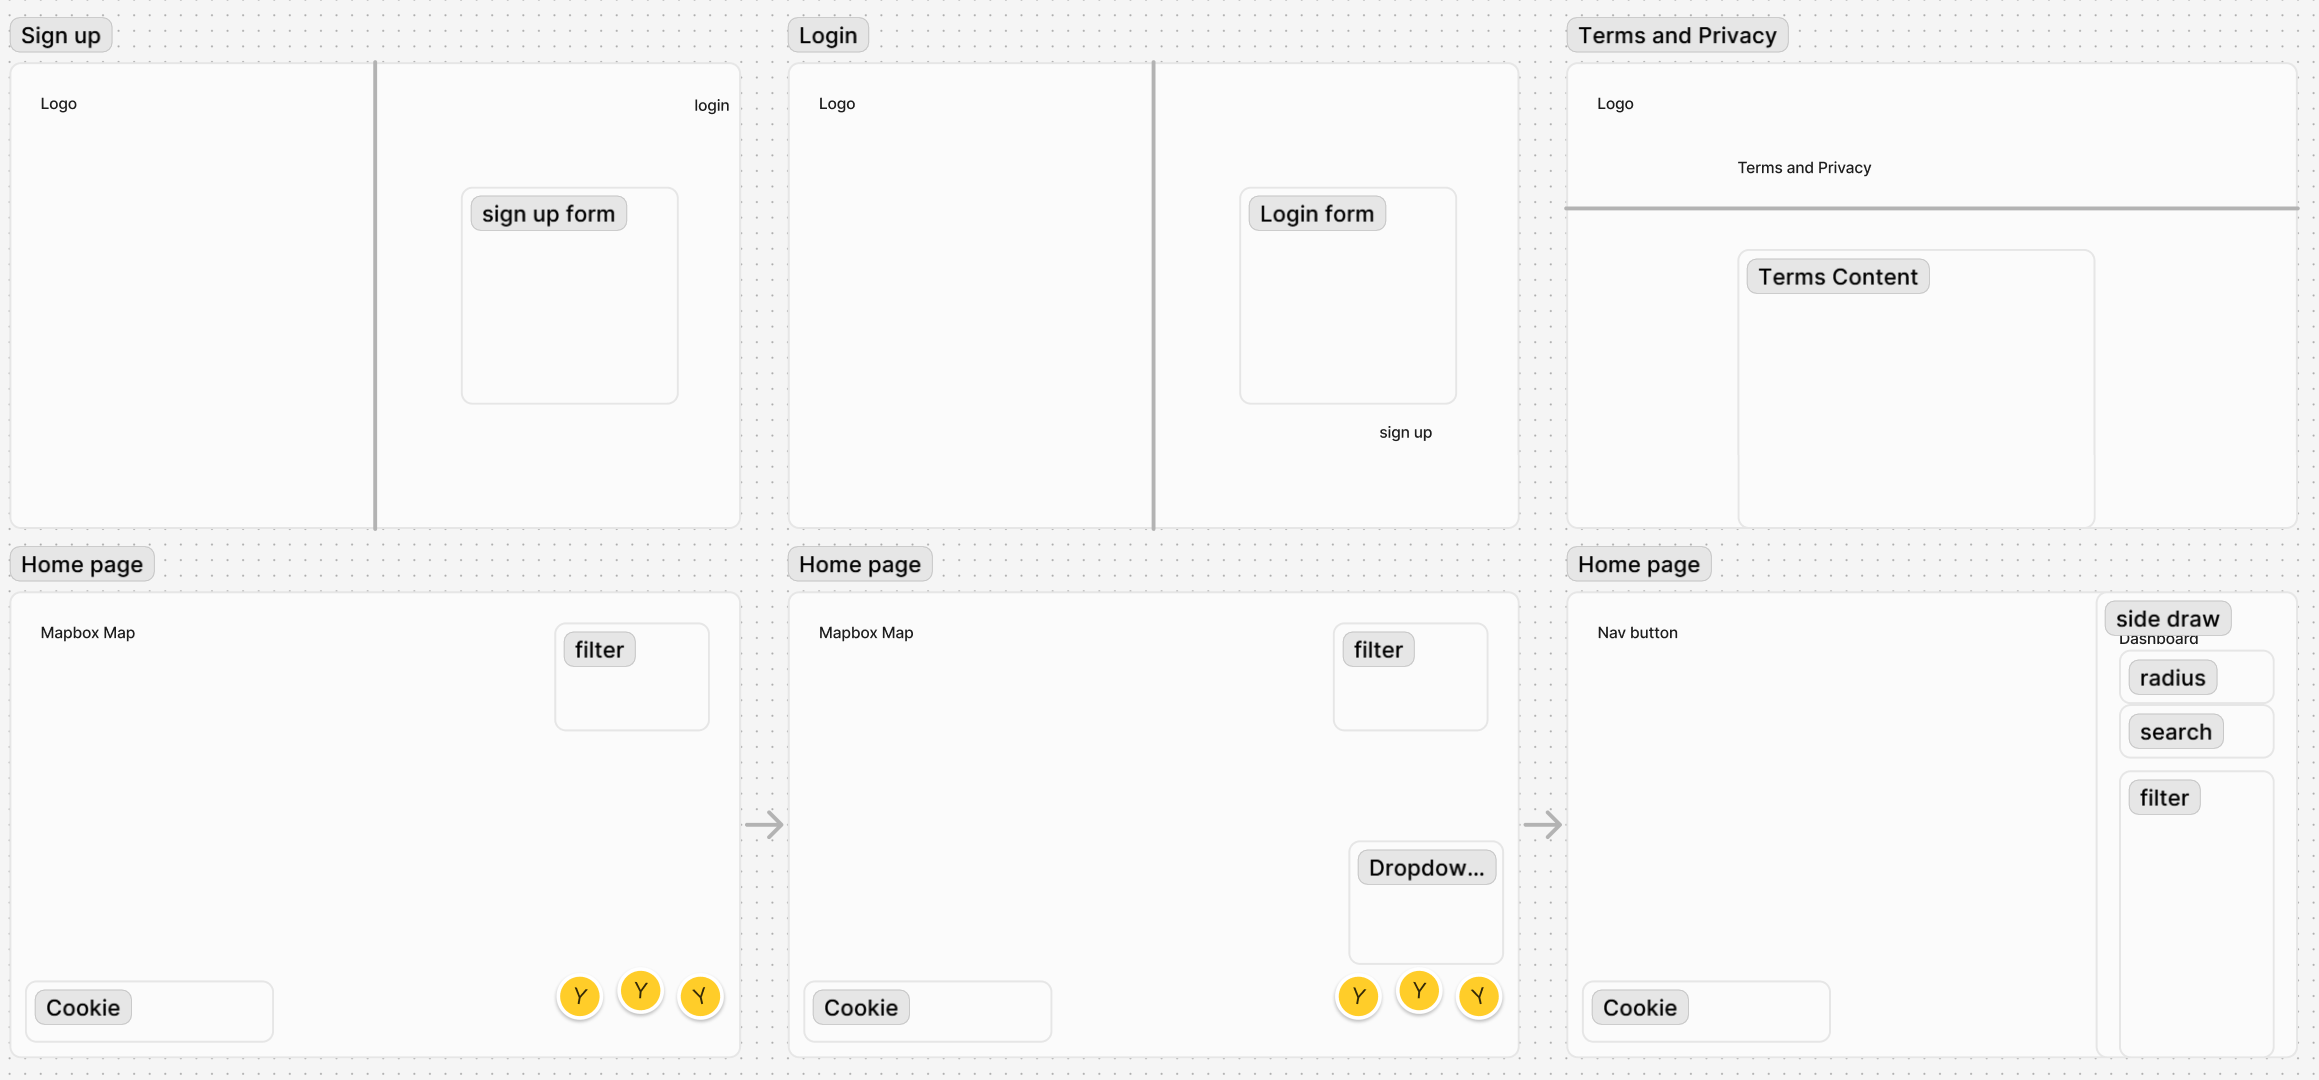
\includegraphics[width=0.48\textwidth]{images/sketch.jpg}
    \caption{Evolution of interface design from initial card-based layout to consolidated dashboard approach}
    \label{fig:prototype-evolution}
\end{figure}

\paragraph{This evolution in our design approach demonstrates the value of iterative prototyping in achieving a balance between functionality and visual clarity. The final layout creates a more focused user experience while maintaining all essential features in an intuitive, accessible format.}

\item \textbf{Wireframe}
\paragraph{Wireframe as a low-fidelity tool, unlike sketches, wireframes show the structure of an interface design, but often lack detail or colour. We also made wireframes of individual pages to build on, such as the home page and the login/signup page in Figure~\ref{fig:wireframe-home} and Figure~\ref{fig:wireframe-signup}, which lay out the structure of the prototype.}
\begin{figure}[h]
    \centering
    \begin{minipage}{0.48\textwidth}
        \centering
        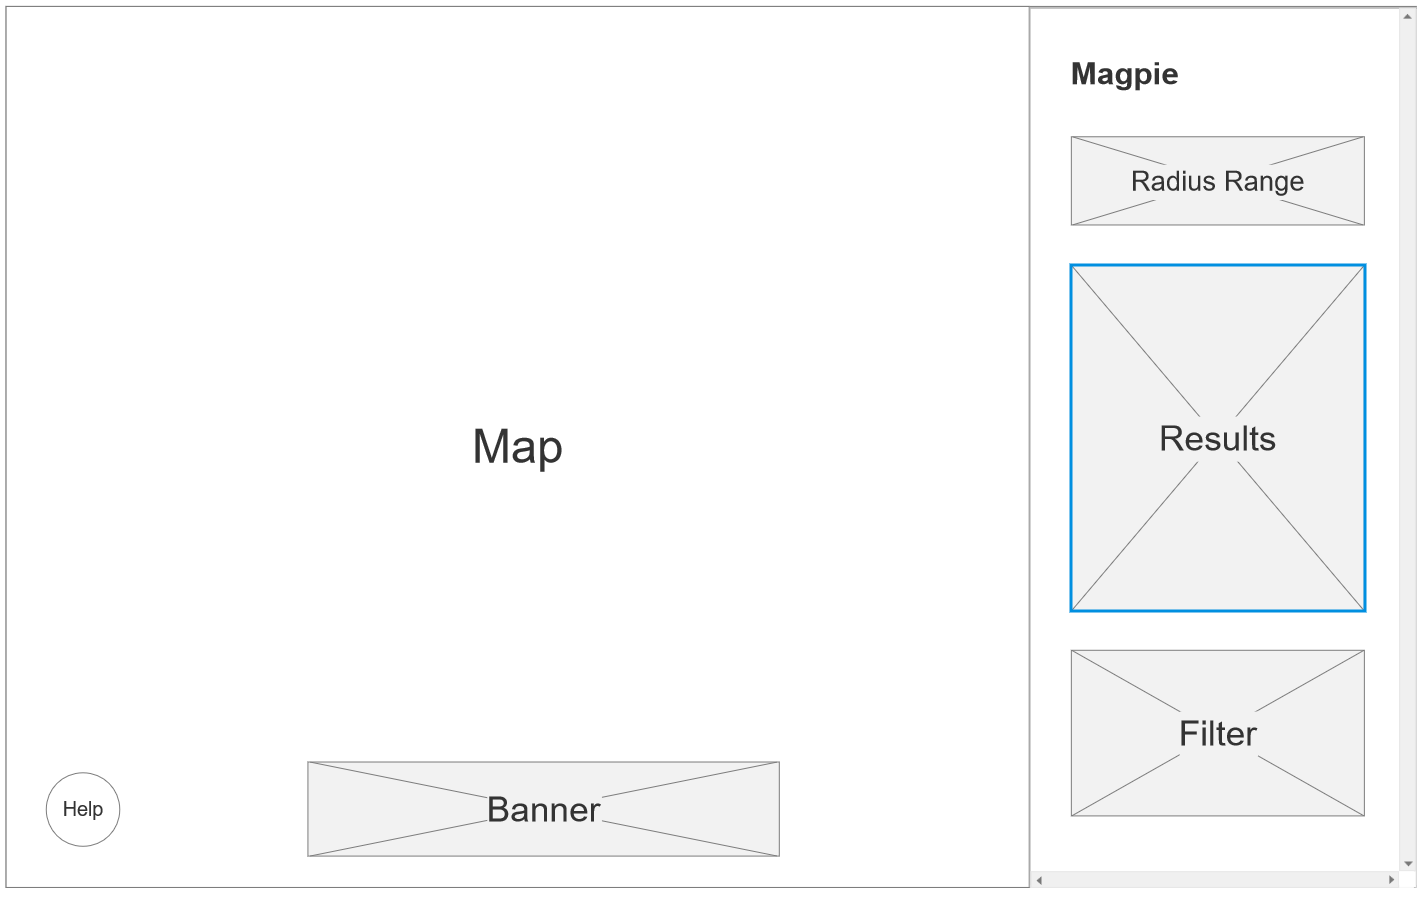
\includegraphics[width=\textwidth]{images/wireframe-home.jpg}
        \caption{Wireframe-home}
        \label{fig:wireframe-home}
    \end{minipage}
    \hfill
    \begin{minipage}{0.48\textwidth}
        \centering
        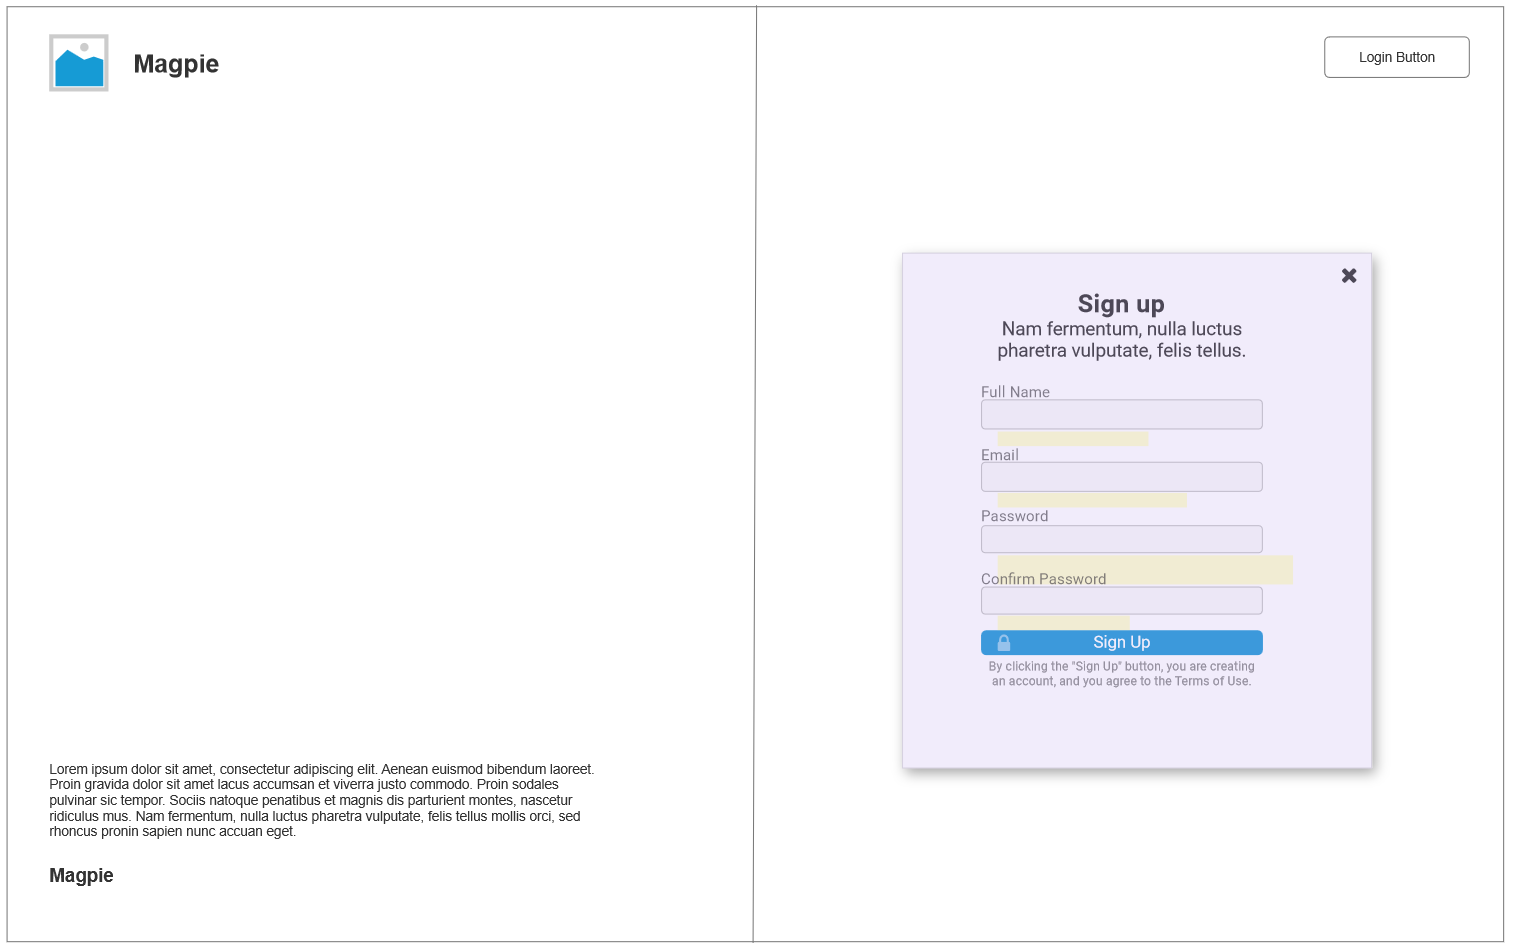
\includegraphics[width=\textwidth]{images/wireframe-signup.jpg}
        \caption{Wireframe-login/signup}
        \label{fig:wireframe-signup}
    \end{minipage}
\end{figure}

\subsection{Medium and High Fidelity Prototyping}
Medium-fidelity prototypes offer more detail, serving as a transitional phase between initial ideas and advanced user testing.

As we move from medium to high fidelity, the prototypes become more refined and detailed, incorporating more realistic interactions and visual elements. This transition allows us to test more specific aspects of the user experience and gather more precise feedback.

High-fidelity prototypes closely resemble the final product in both form and function.


\subsection{User Interface Iteration}
Our iterative UI process focuses on the overall process involved in the User Interface (UI) and User Experience (UX). For example, the visual and interactive components that users use, including buttons, icons, and layouts, while UX covers the overall journey and emotional response of the user during an interaction. The importance of good UI and UX design lies in the improvement of user satisfaction, which then links to better customer retention and enterprise success. It is believed, through studies, that well-thought-out user experiences can increase retention manyfold.\cite{psycray2023} We did extensive reviews of each and every aspect in our iterations-from color scheme and typography to layout and how the navigation structures work-to ensure usability and interactivity. In terms of visual elements, we used a single colour scheme of predominantly black to create a cohesive and less intrusive design. In addition to cultural considerations, the colour black is also inclusive and has a wide audience. The contrast between the accessible text and the background is also stronger, with enough contrast to improve readability for the user.

\paragraph{Iteration 1:}

Our first iteration used the same design as sketch, but it was more cluttered aesthetically and consistently. The fragmented card-based design made the ribbon look complicated and overwhelming for users. And the first version didn't have a better dashboard. The login/signup page adopts the original shadcn style, which needs to be customized and improved.

\begin{figure}[h]
    \centering
    \begin{minipage}{0.48\textwidth}
        \centering
        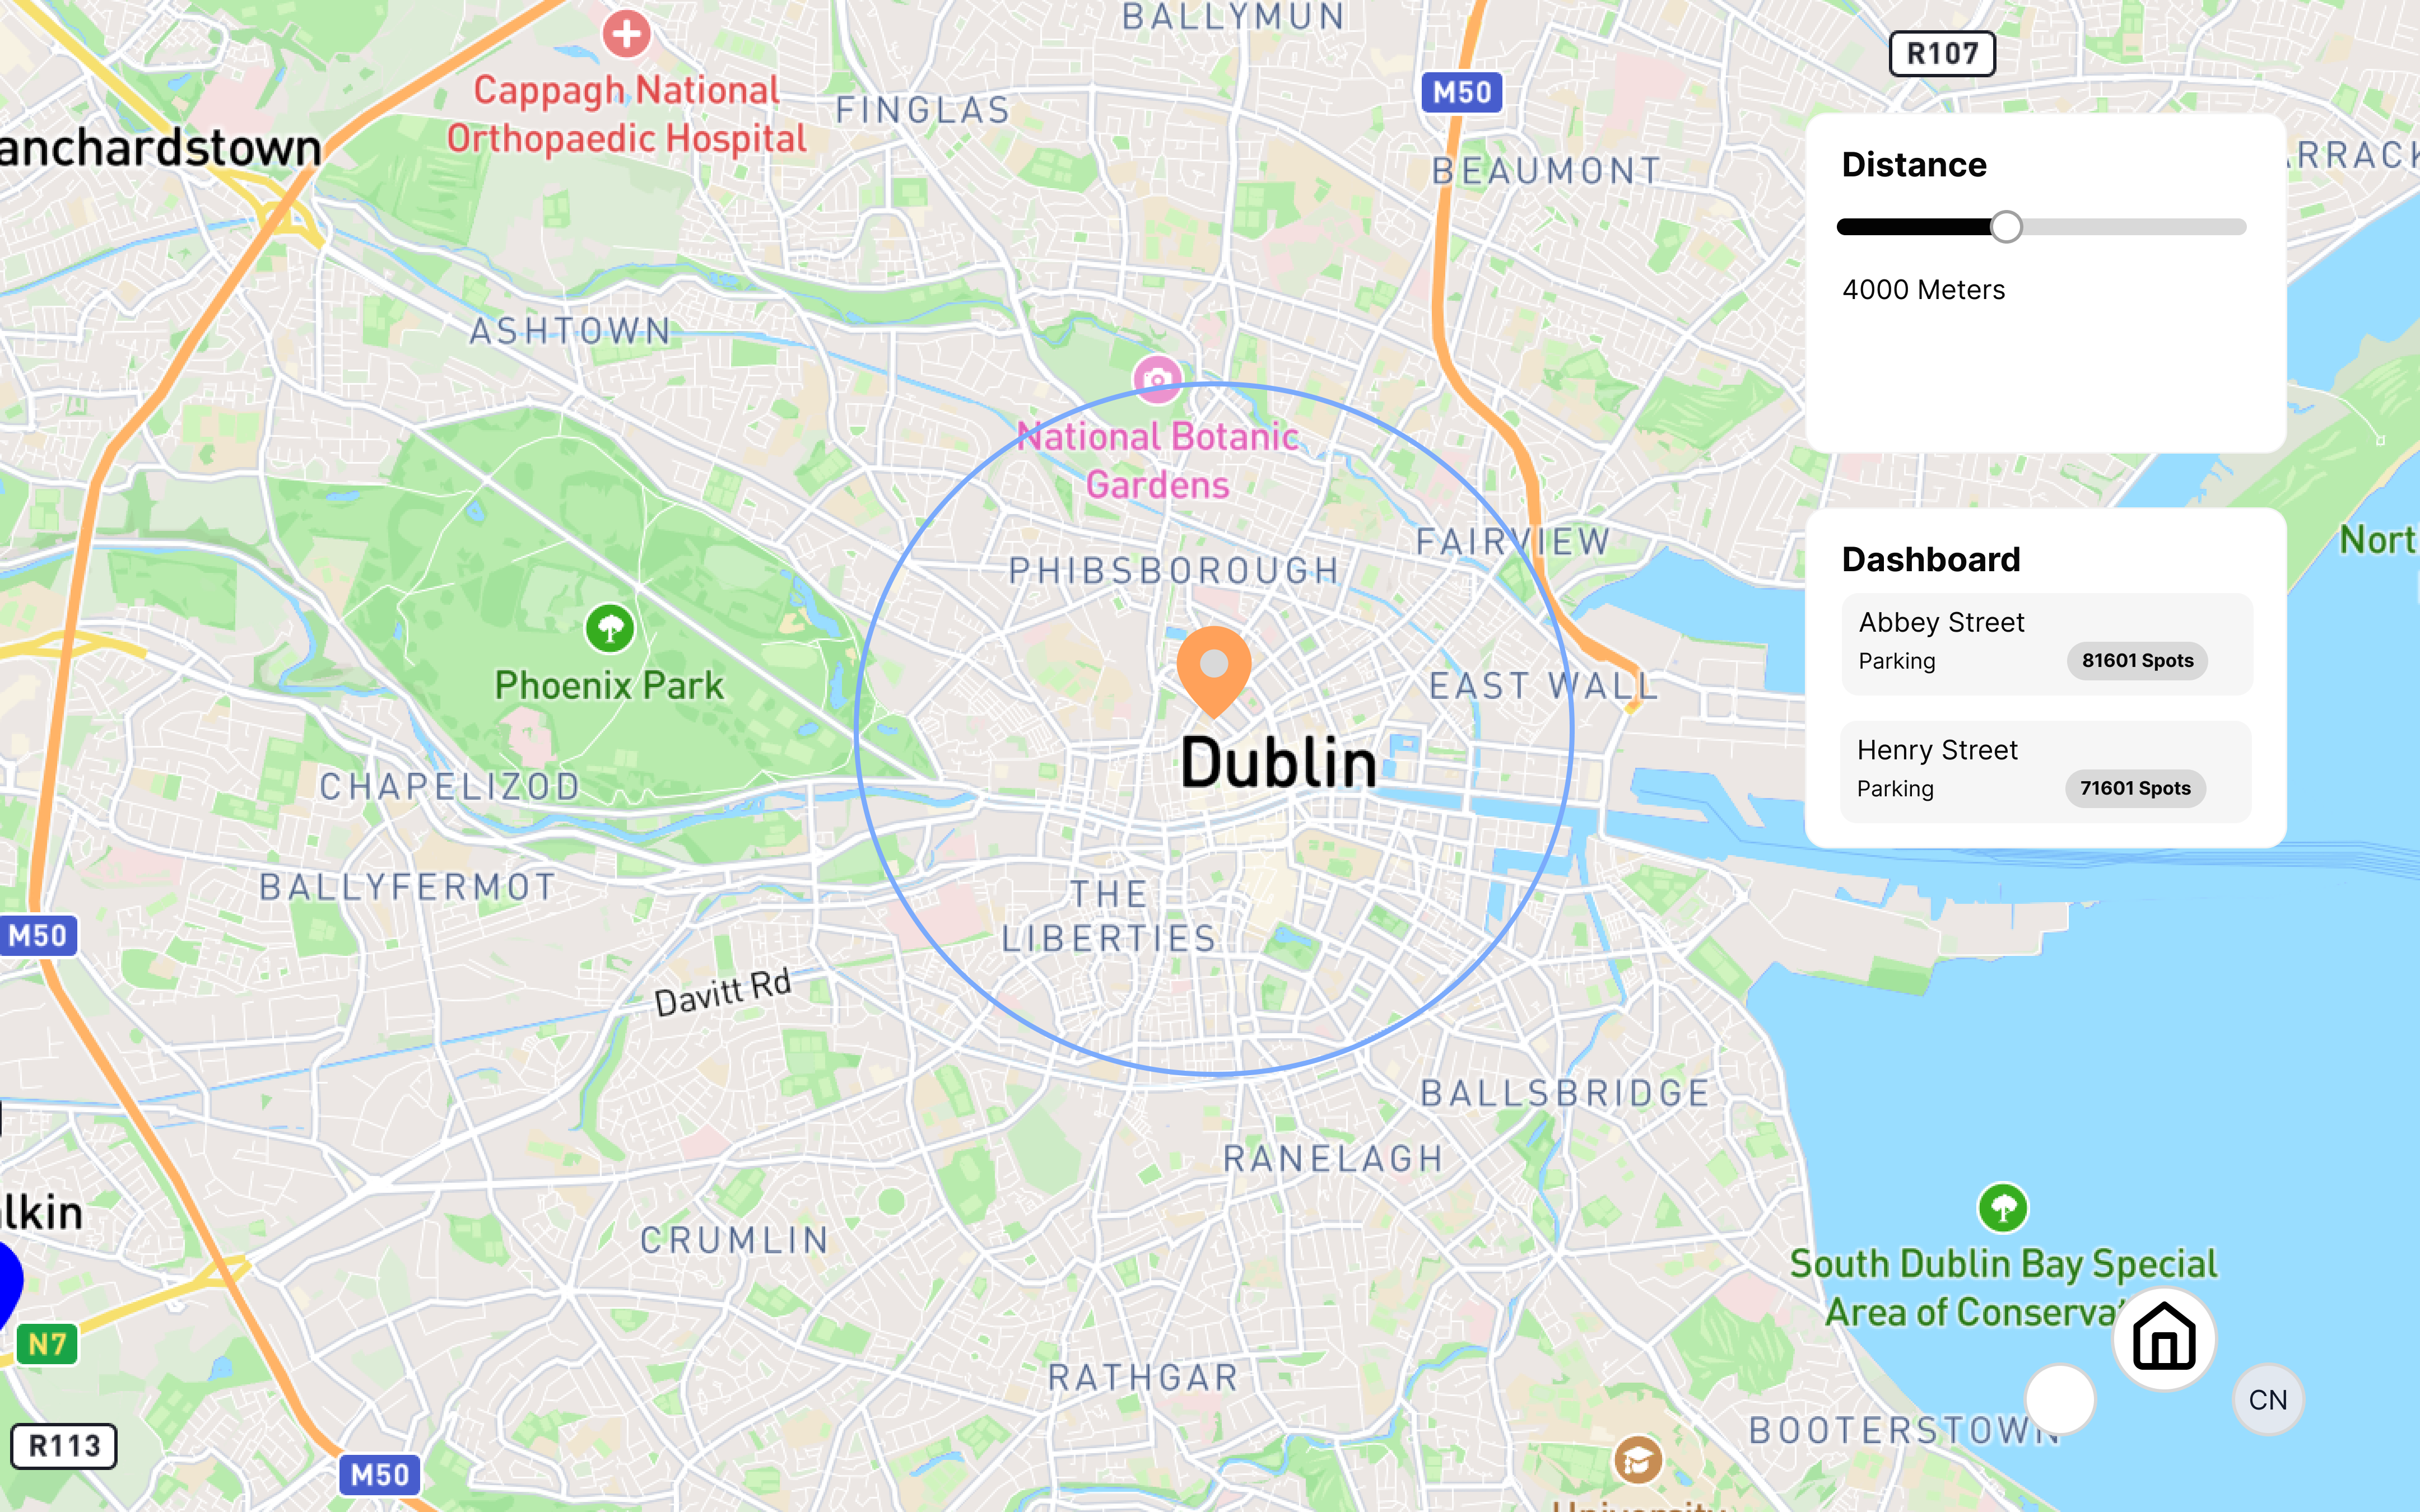
\includegraphics[width=\textwidth]{images/v1_Home Page.png}
        \caption{v1_Home Page}
        \label{fig:v1_Home Page}
    \end{minipage}
    \hfill
    \begin{minipage}{0.48\textwidth}
        \centering
        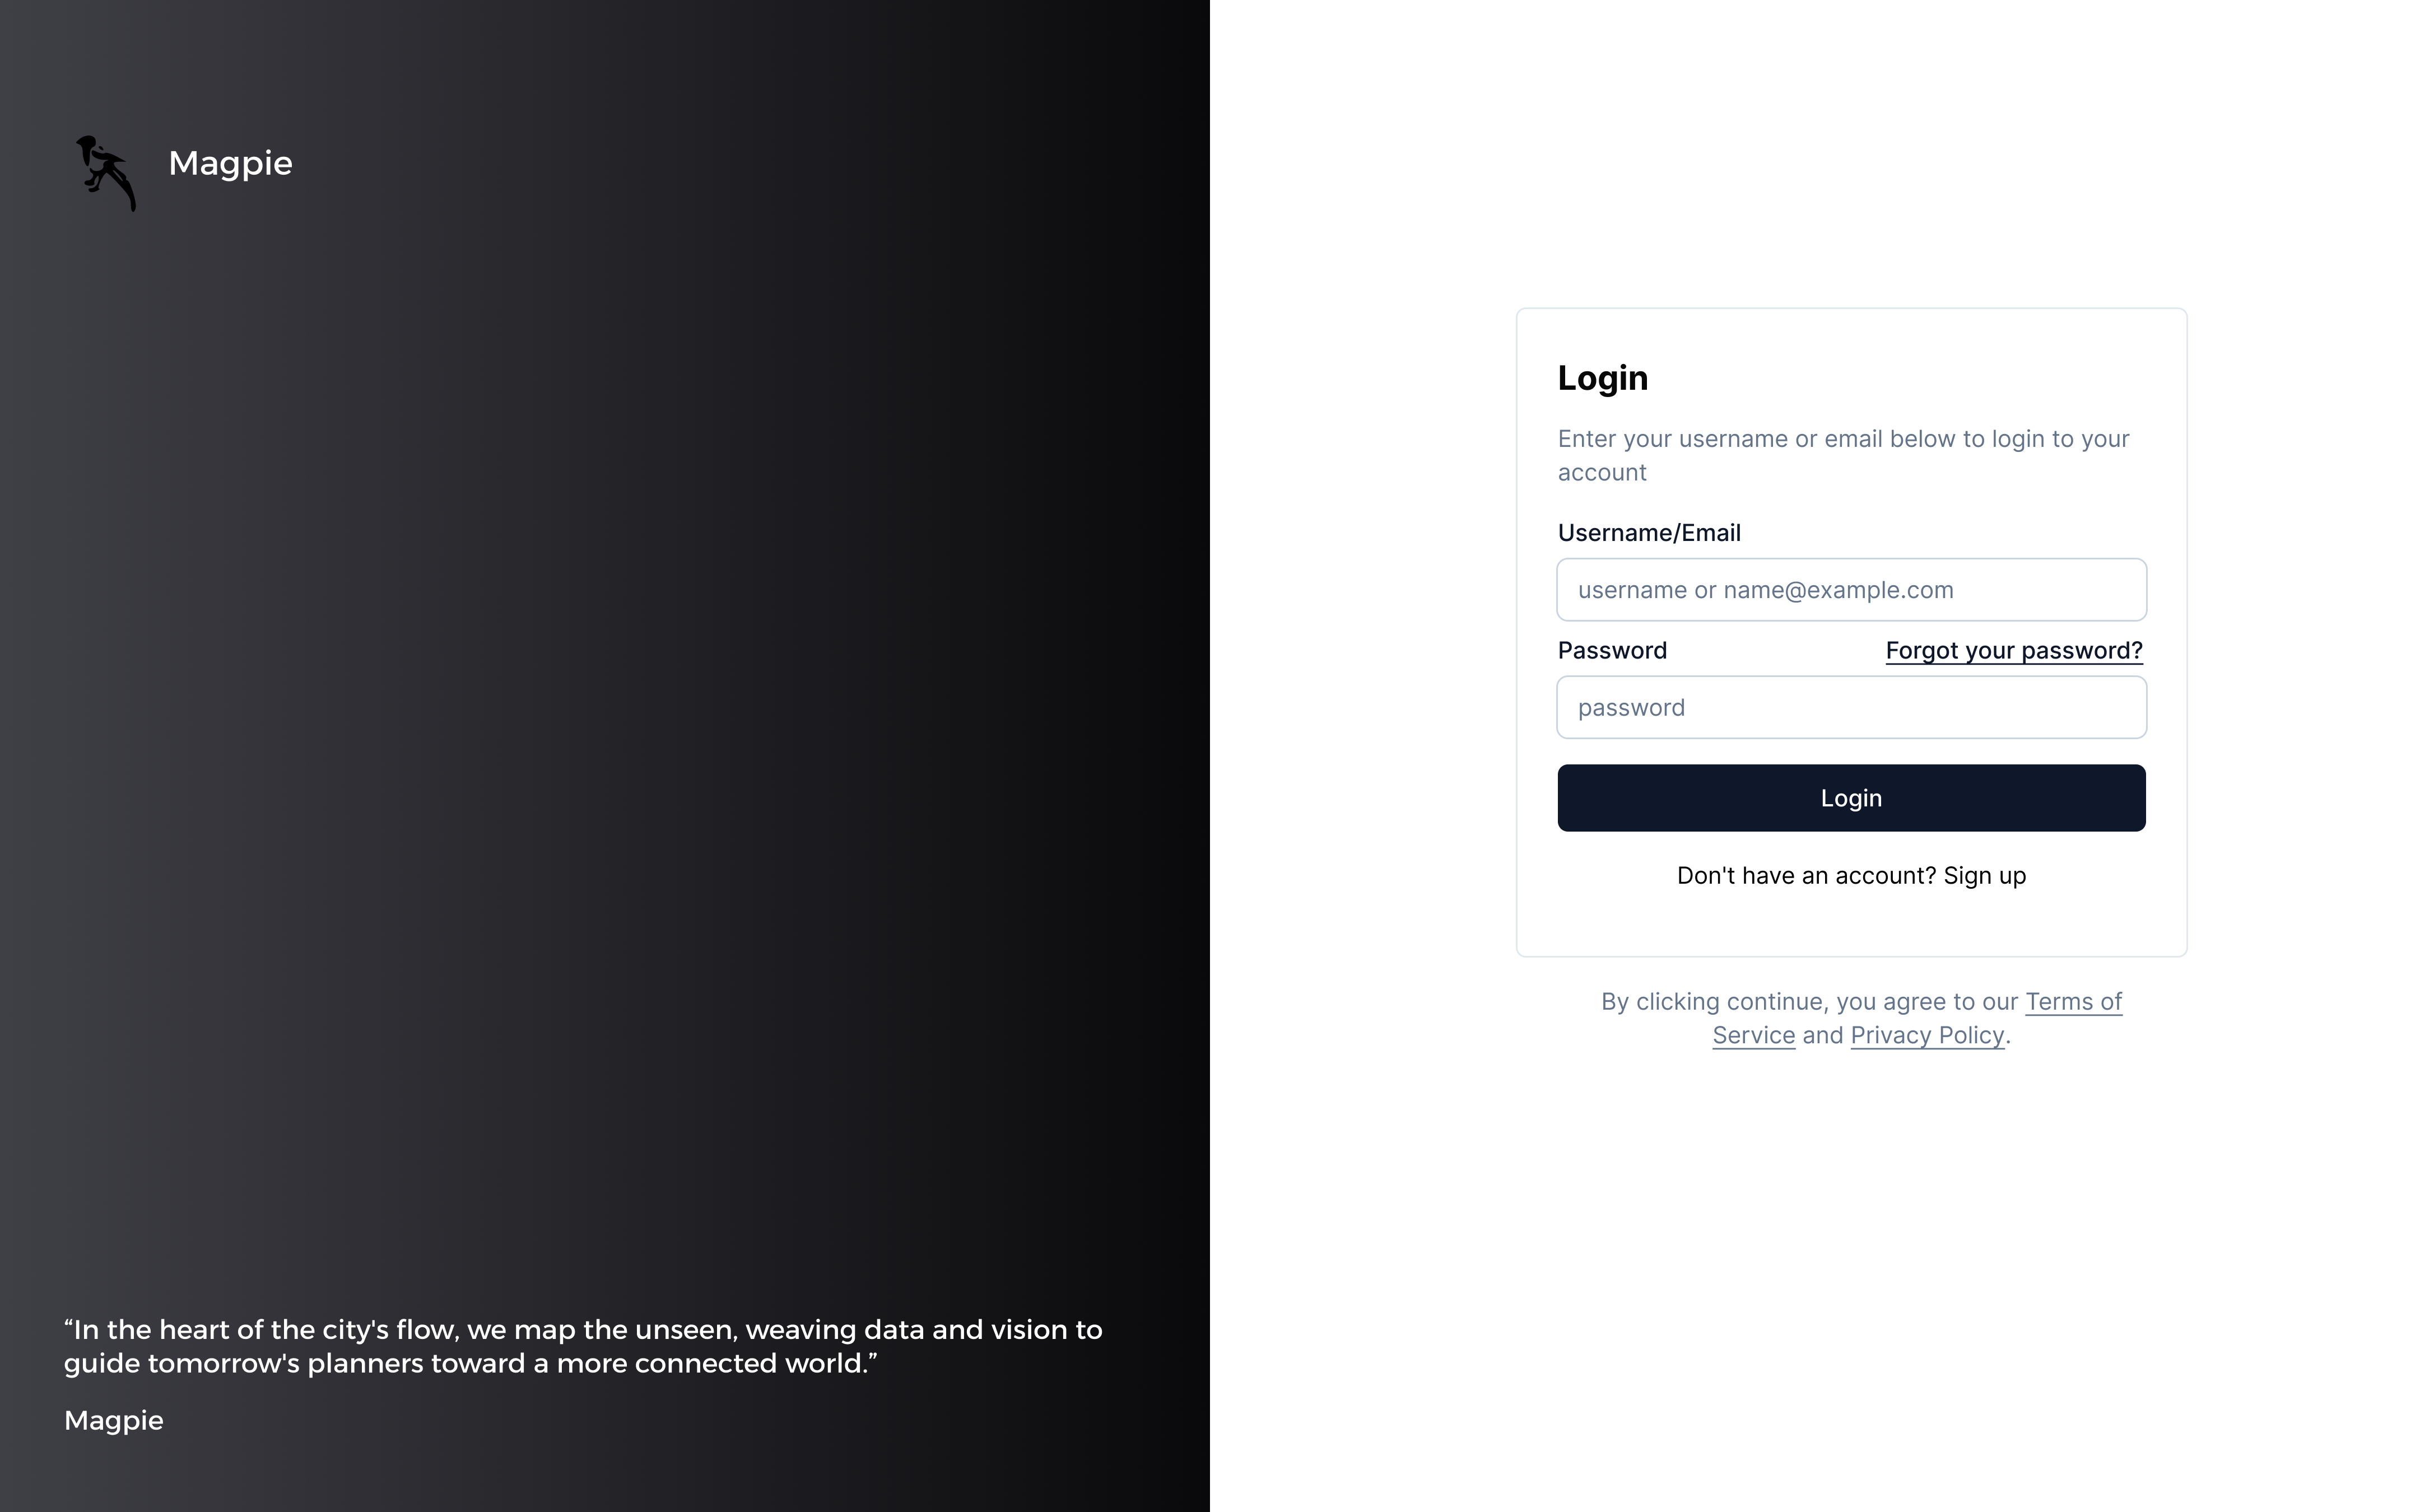
\includegraphics[width=\textwidth]{images/v1_Login.png}
        \caption{login/signup}
        \label{fig:v1_Login}
    \end{minipage}
\end{figure}


\paragraph{Iteration 2:}
In the second version, we introduced the search bar in the initial stage and integrated each card into the dashboard bar on the right. In the later iterations, we also integrated the search bar to the right, making our structure clearer. In terms of interactivity, we ensured that buttons and sliders were easy to use and responded to user operations intuitively. The amenity filter in the second version used checkboxes, but it was not user-friendly.

\begin{figure}[h]
    \centering
    \begin{minipage}{0.48\textwidth}
        \centering
        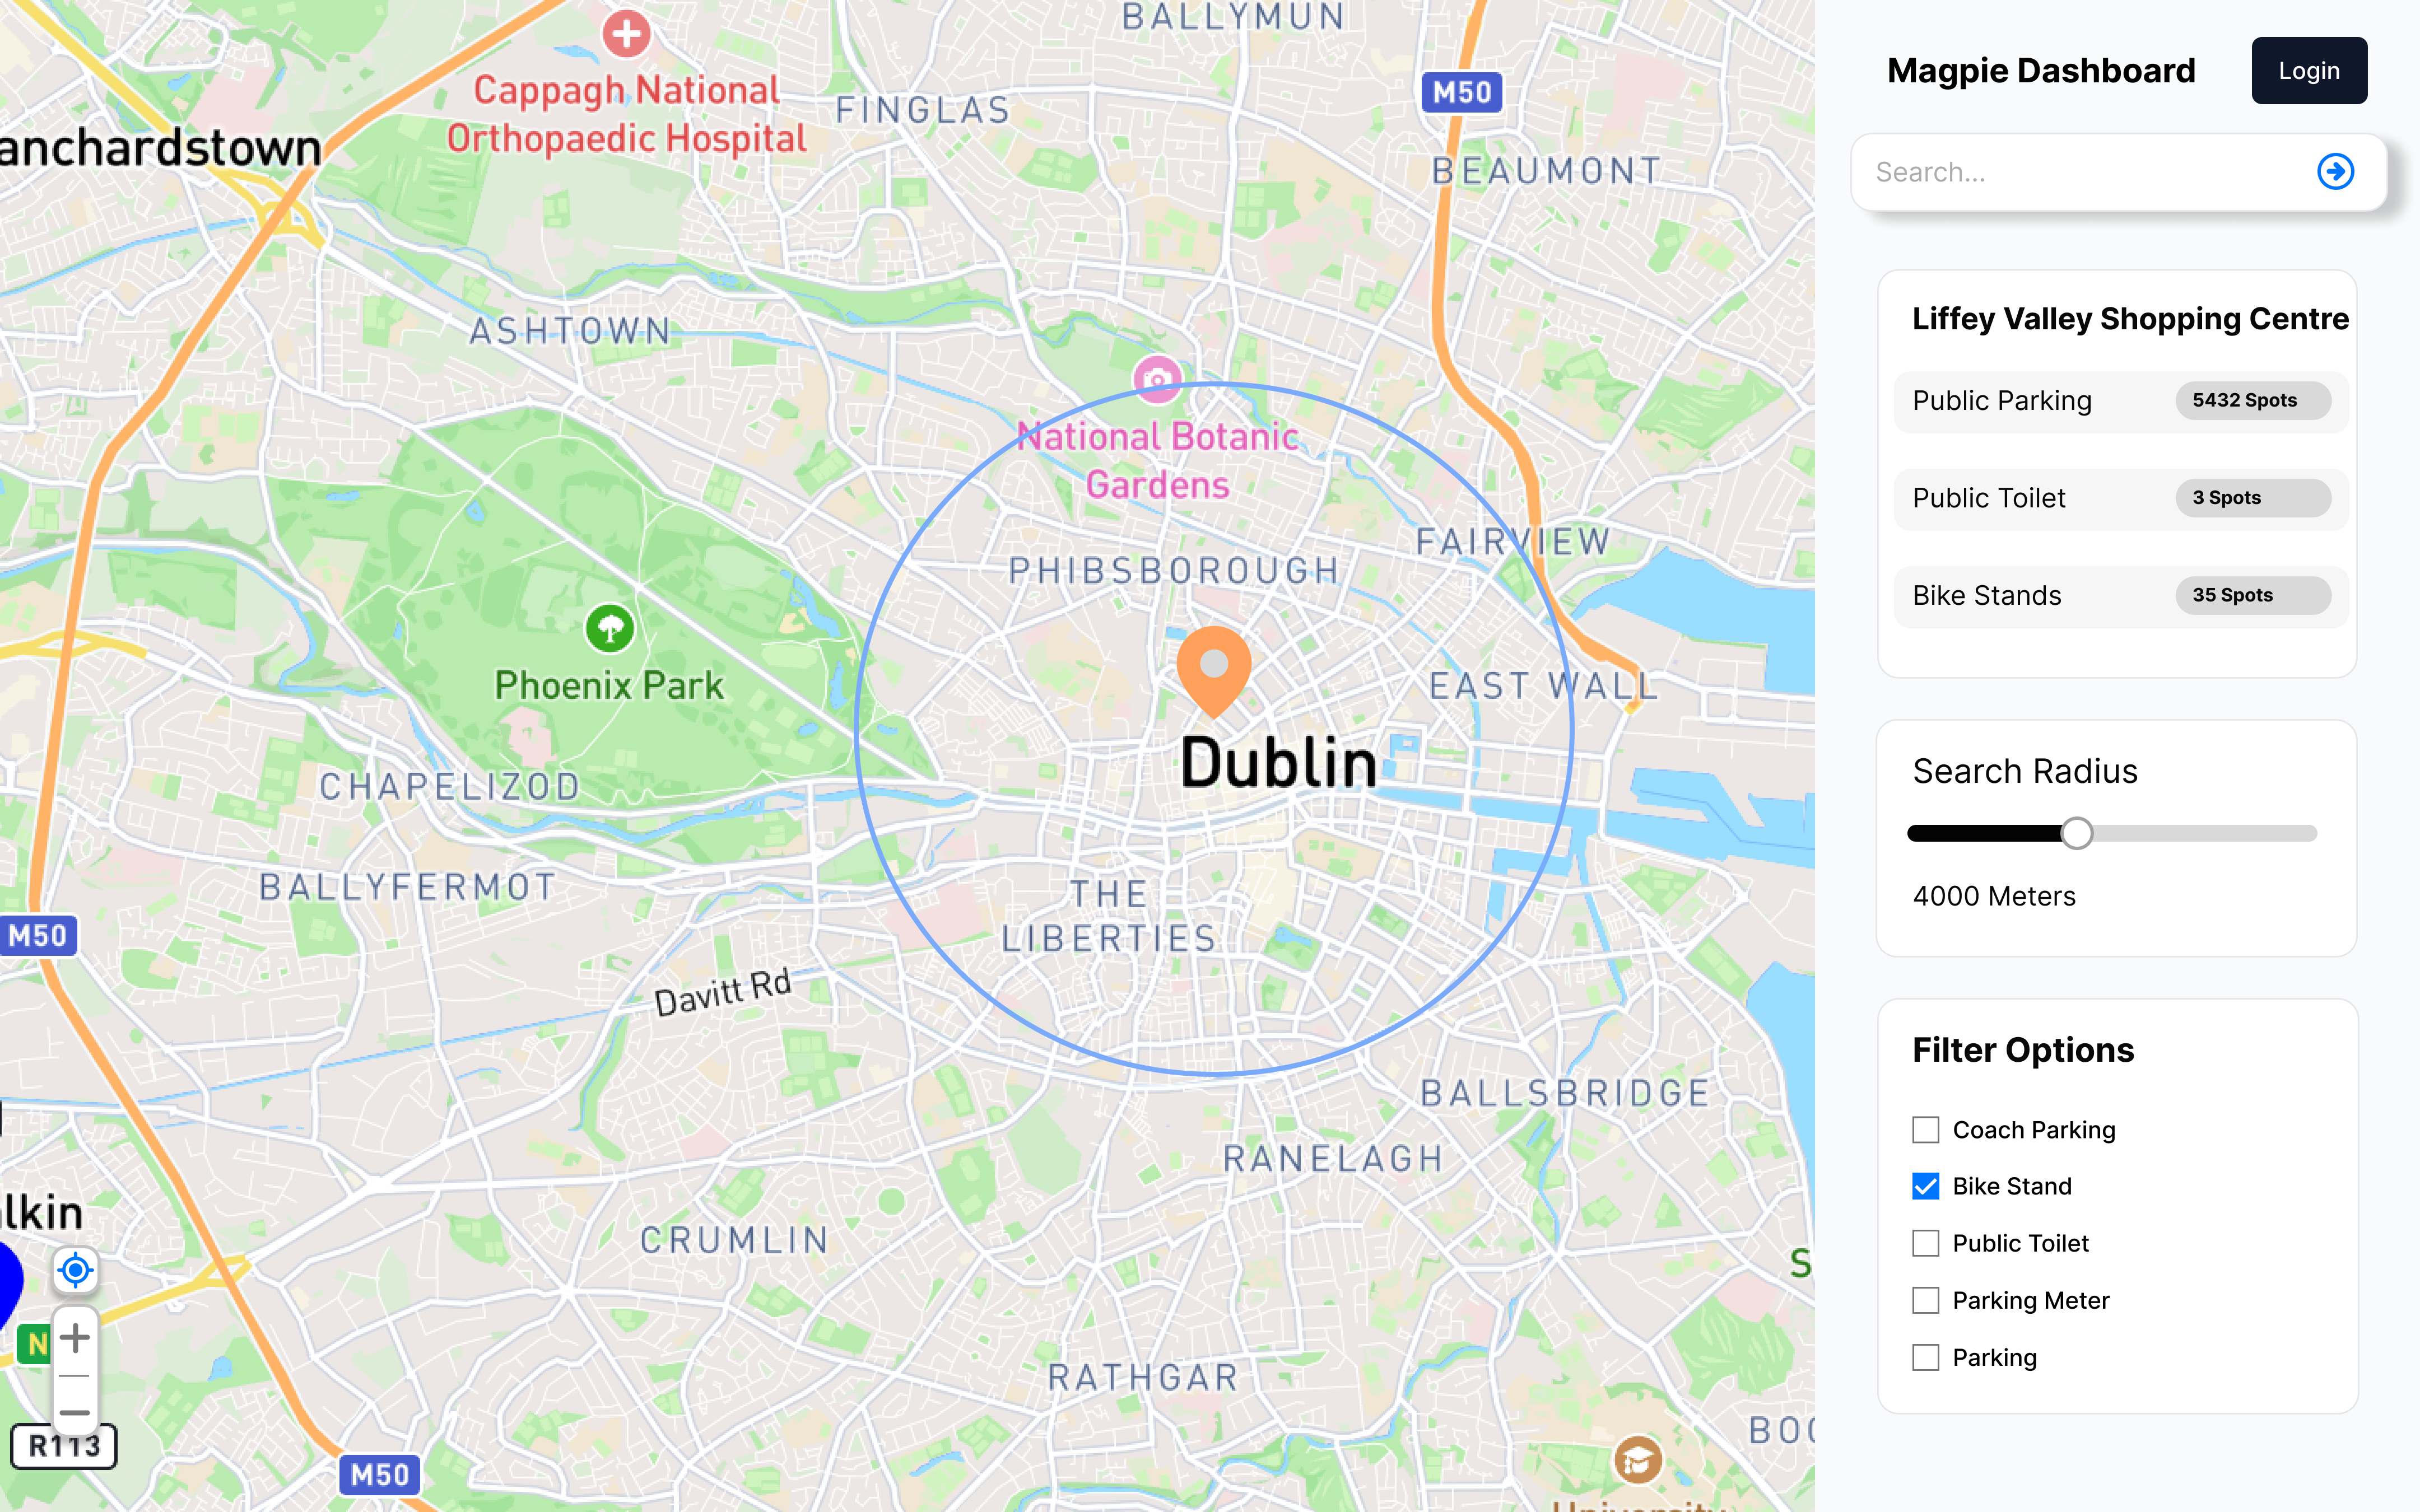
\includegraphics[width=\textwidth]{images/v2_Home Page.png}
        \caption{v2_Home Page}
        \label{fig:v2_Home Page}
    \end{minipage}
\end{figure}


\paragraph{Iteration 3:}
For version 3 we have added a onboarding tutorial step to the design, which allows new users to quickly familiarise themselves with the app and creates a clear and intuitive interface that guides the user through the interactions. In addition we added updates to the history page, term and privacy page.Home pageWe tried to use the drop down menu option to select amenity to display filters, but through user surveys, we found that the interaction between filters and results was not good, and the drop down menu also added complexity. Also some professional users have suggested that the icon is not visible on the map, so the icon will be updated in the fourth iteration.
\begin{figure}[h]
    \centering
    \begin{minipage}{0.32\textwidth}
        \centering
        \includegraphics[width=\textwidth]{images/v3_Home Page.png}
        \caption{v3_Home Page}
        \label{fig:v3_Home Page}
    \end{minipage}
    \hfill
    \begin{minipage}{0.32\textwidth}
        \centering
        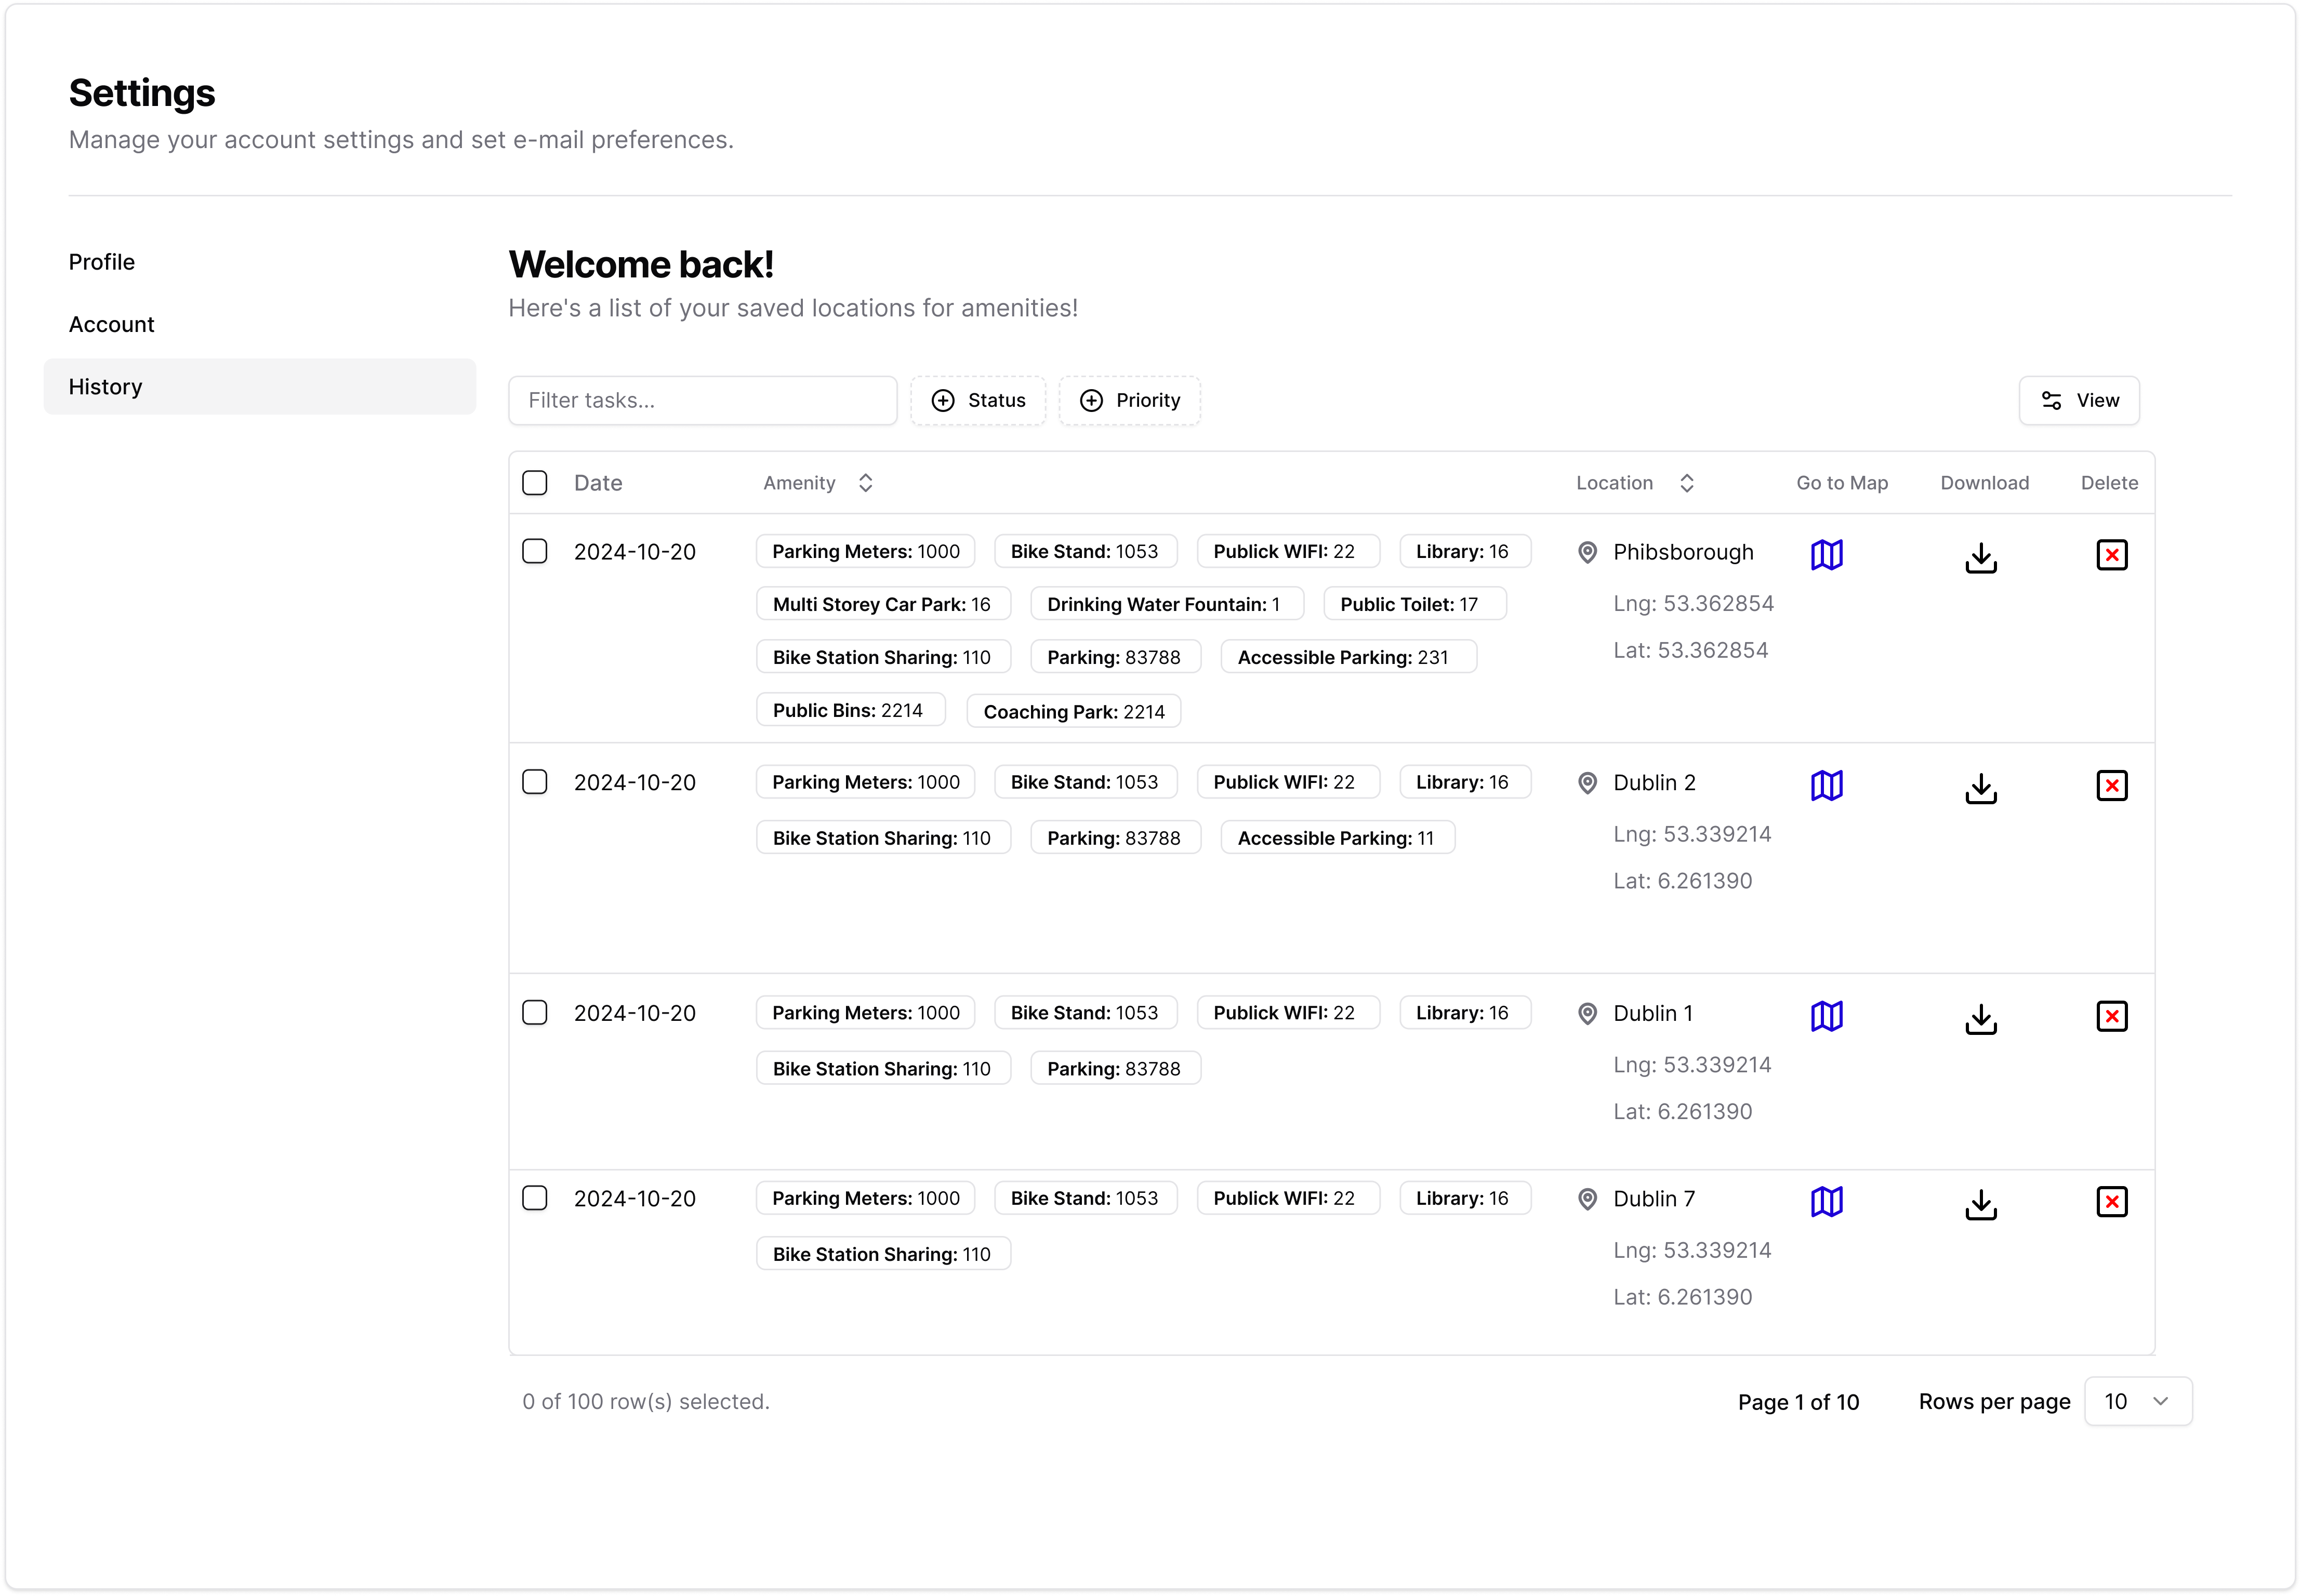
\includegraphics[width=\textwidth]{images/v3_History.png}
        \caption{v3_History}
        \label{fig:v3_History}
    \end{minipage}
    \hfill
    \begin{minipage}{0.32\textwidth}
        \centering
        \includegraphics[width=\textwidth]{images/v3_onboarding.png}
        \caption{v3_onboarding}
        \label{fig:v3_onboarding}
    \end{minipage}

\end{figure}



\paragraph{Iteration 4:}
For version 4 we have made some major changes to the front end. First of all, the icon has become more understandable and the colours are more differentiated, each amenity is in a different spectrum of colours and can be seen more clearly. The dropdown menu of the third version was cancelled in the fourth version, the burger menu would make the user can not find the corresponding function buttons, so we expanded them so that you can directly click the history entrance and onboarding button. In addition, according to the feedback from professionals, we also added zoom function and designed scale ruler and export image function. Due to time constraints, the latter two were not fully implemented, and the Search function was gathered together on the right side above the dashboard, with more clickable range options such as ‘100m’, ‘200m’, and so on. Filter is a very important component, now you can click on the small eyes to enable the corresponding amenity, which is more intuitive and interactive. In addition, we have created a landing page to showcase our project.

\begin{figure}[h]
    \centering
    \begin{minipage}{0.48\textwidth}
        \centering
        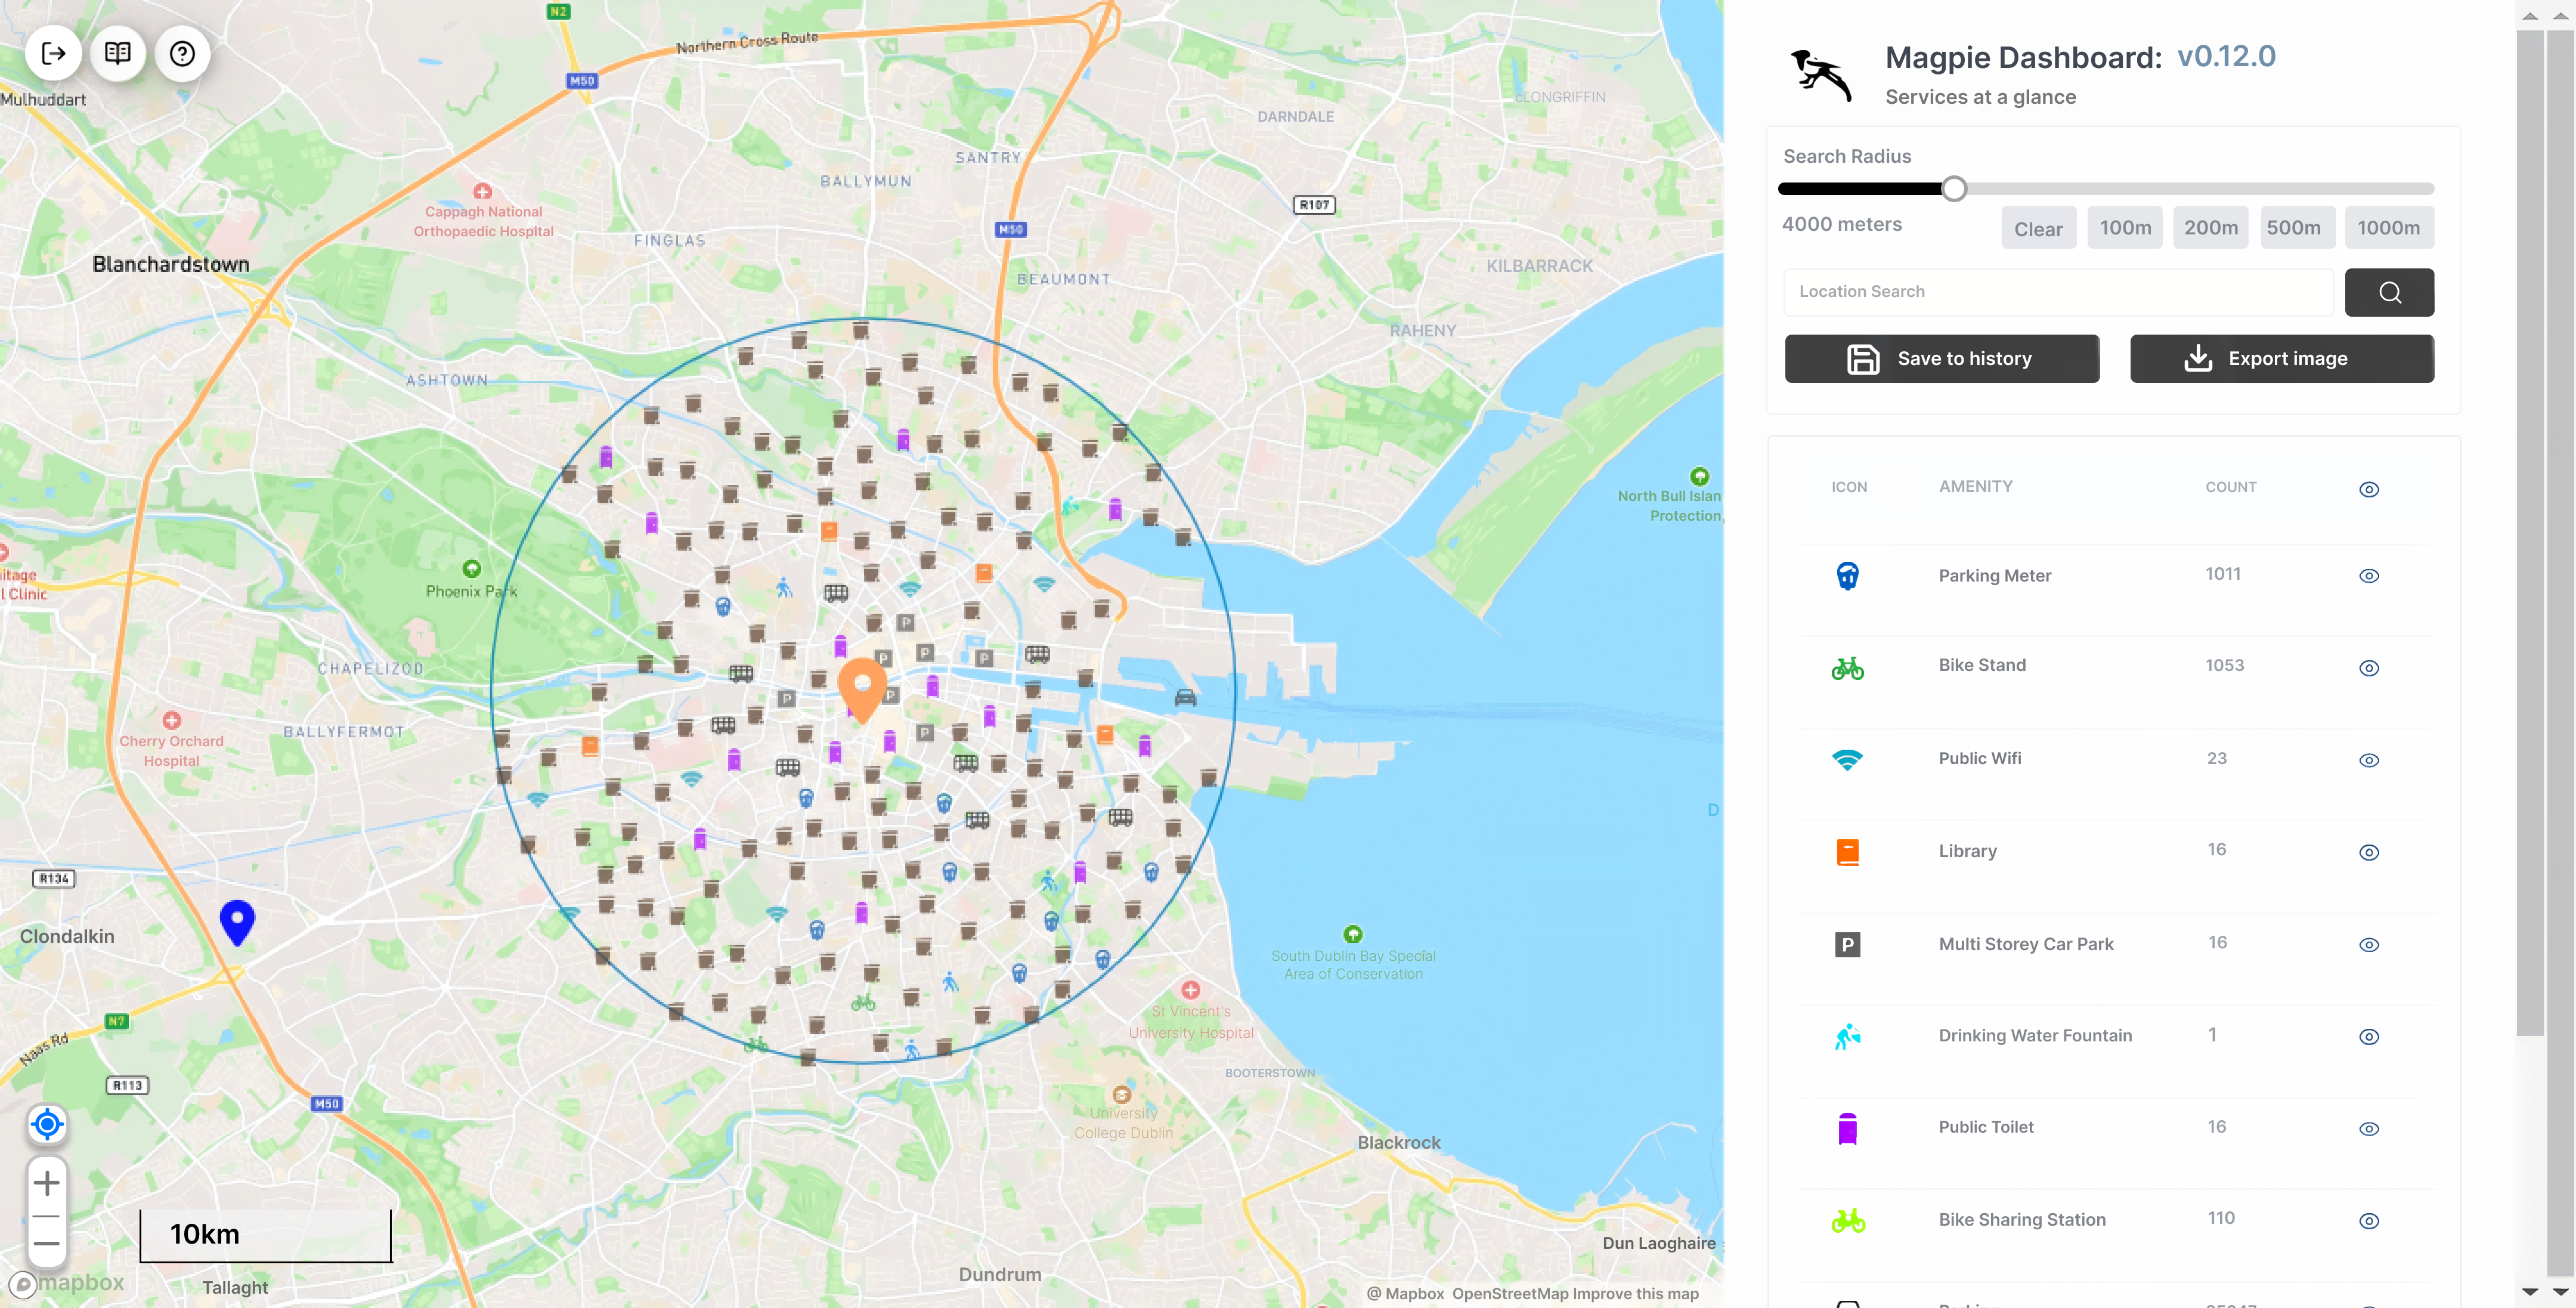
\includegraphics[width=\textwidth]{images/v4_Home.png}
        \caption{v4_Home Page}
        \label{fig:v4_Home Page}
    \end{minipage}
    \hfill
    \begin{minipage}{0.48\textwidth}
        \centering
        \includegraphics[width=\textwidth]{images/v4_Landing Page.png}
        \caption{v4_Landing Page}
        \label{fig:v4_Landing Page}
    \end{minipage}
\end{figure}
